\documentclass{standalone}
\usepackage{tikz}

\begin{document}

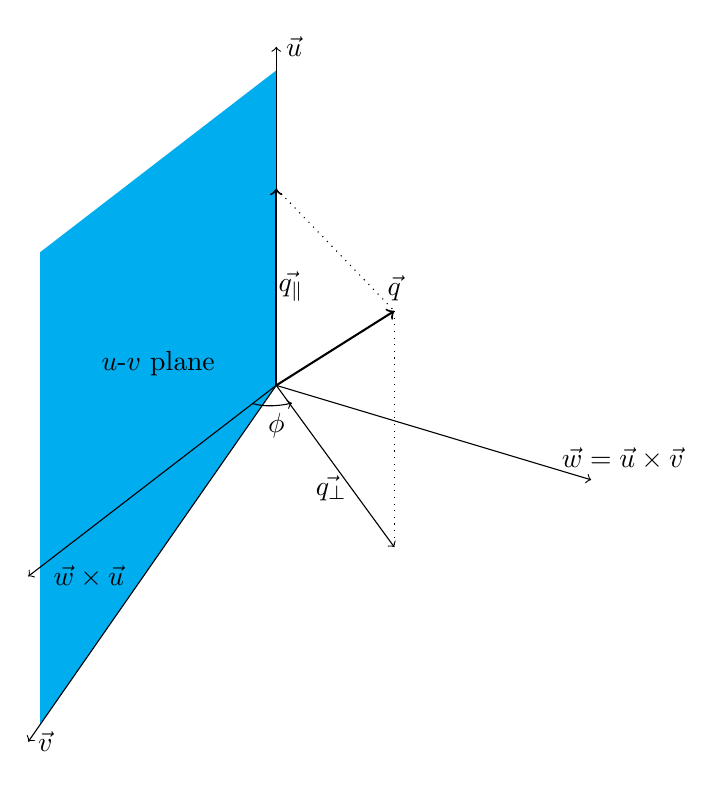
\begin{tikzpicture}[x={(-5mm,-3.85mm)},z={(0,1cm)},y={(1cm,-.3cm)}]
  \path [fill=cyan] (0,0,0)--(6,0,-2)--(6,0,4)--(0,0,4) node [above,xshift=-1.5cm,yshift=-4cm] {$u$-$v$ plane};

  \draw [->] (0,0) -- (6.3,0,-2.1) node [right] {$\vec{v}$};
  \draw [->] (0,0) -- (0,4,0) node [above,xshift=0.4cm] {$\vec{w} = \vec{u} \times \vec{v}$};
  \draw [->] (0,0) -- (0,0,4.3) node [right] {$\vec{u}$};

  \draw [->] (0,0) -- (6.3,0,0) node [right,xshift=0.2cm] {$\vec{w} \times \vec{u}$};

  \draw [dotted] (0,0,2.5) -- (3,3,3);

  \draw [->,line width=0.75pt] (0,0,0) -- (3,3,3) node [above] {$\vec{q}$};
  \draw [dotted] (3,3,3) -- (3,3,0);
  \draw [->] (0,0,0) -- (3,3,0)  node [midway,below,xshift=-0.05cm] {$\vec{q_{\perp}}$};
  \draw [->,line width=0.7pt] (0,0,0) -- (0,0,2.5) node [midway,right,xshift=-0.1cm] {$\vec{q_{\|}}$};

  \draw [->] (0.6,0,0) arc [start angle=0,end angle=45,x radius=1,y radius=0.5] node [below,xshift=-0.2cm] {$\phi{}$};

\end{tikzpicture}

\end{document}
1
